\section{Zero-body acquisition controls}
\label{app:acquisition}

The original pilots do not distinguish acquisition, retention and readout.
Three subsequent, separately frozen local CPU discovery protocols test native
recall before a distractor body is introduced. Both use seed 0, GRU hidden
state 128 or LSTM complete state $[h,c]$ of dimension 256, encoder width 64,
batch size 32 and native FP32. A full-prefix $R=0$ episode has sixteen ordered
independent WRITEs followed by a QUERY selecting one of addresses 0--7; the
eight later WRITEs are nuisance inputs. QUERY carries no payload.

\paragraph{The discovery grid fails before body training.}
The twelve-fit GRU/LSTM $\times$ categorical/continuous $\times$
learning-rate grid $\{0.0005,0.001,0.003\}$ completes 10,200 updates.
Two categorical fits fail their 100-update fixed-batch diagnostic. The other
ten pass immediate WRITE--QUERY recall, then fail the full-prefix $R=0$ gate
after 1,000 updates. No eligible checkpoint or learning rate is selected.
This is a schedule-specific acquisition audit, not an impossibility result.

\paragraph{Equal subsequent prefix exposure does not produce full competence.}
A distinct eight-fit protocol compares fresh initialization against transfer
from the pinned immediate-task step-500 weights, resetting AdamW in both
conditions. Transfer has 500 additional historical immediate-task updates;
the comparison equalizes only subsequent $R=0$ exposure. All fits complete
exactly 5,000 prefix updates at learning rate 0.001, weight decay 0.01 and
gradient clipping 1. They share the complete training stream within each task.
Every scheduled checkpoint is retained; no earlier success or minimum-loss
checkpoint replaces the fixed endpoint.

\begin{figure}[htbp]
\centering
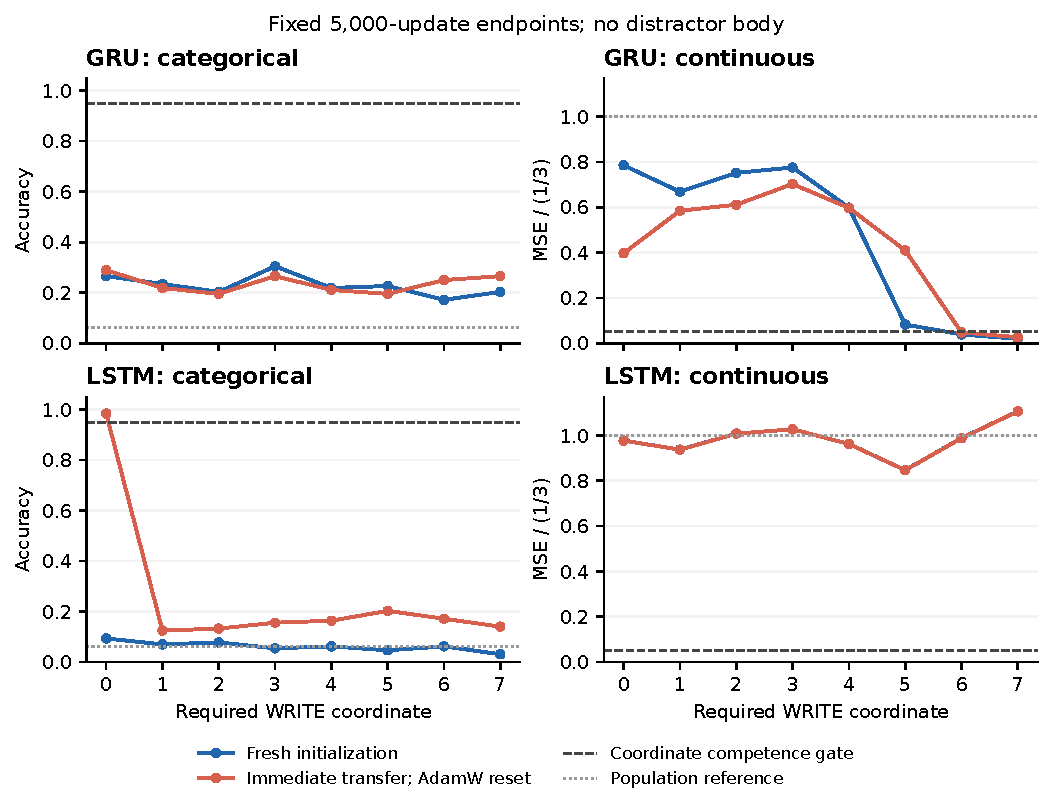
\includegraphics[width=0.92\linewidth]{../doc/auto/figures/prefix-acquisition-v3-endpoints.pdf}
\caption{\textbf{Partial acquisition fails the joint competence requirement.}
Every point uses 128 validation episodes for one required coordinate at the
fixed 5,000-update endpoint. Identical $R=0$ arms are displayed once. Blue is
fresh initialization; orange transfers fixed step-500 immediate-task weights
with a new AdamW optimizer. Dashed lines mark accuracy 0.95 or MSE$/ (1/3)$
0.05. Dotted lines are the uniform-classifier and population zero-predictor
references; the continuous reference is not the realized-sample baseline.
Coordinates and conditions are repeated measurements of training seed 0,
without independent training-seed uncertainty bars. No distractor body is used.}
\label{fig:prefix-acquisition}
\end{figure}

\Cref{fig:prefix-acquisition} retains every coordinate. Both continuous GRU
conditions pass coordinates 6 and 7, and transferred categorical LSTM passes
coordinate 0 with accuracy 0.984375; every other endpoint coordinate fails.
None of the eight endpoints or eighty scheduled validations passes all eight
coordinates. The partial successes prevent an interpretation of universal
failure across coordinates. They do not isolate WRITE lag, address binding,
required memory load or native readout. No covariance-dimension or causal-memory
result is inferred from these native errors.

\paragraph{Provenance and scope.}
The twelve-fit source is
\hash{1add2b6aba948714673f45f1b7854eff6212833d}; the eight-fit source is
\hash{999d88d8679c0f353c6bb7fb4f5ab8433a7e730c}.
The respective configurations are
\path{configs/experiments/competence-recovery-v2.json} and
\path{configs/experiments/prefix-acquisition-discovery-v3.json}.
Validation is frozen before fitting, with fresh v3 sampling seed 20001;
training stream seed is 2026101301. Independent reduction reconciles all
forty thousand v3 update identities, every saved validation and a native
checkpoint replay subset. Exact scalar values, source/stream/checkpoint
hashes, acceptance scope and figure provenance appear in
\path{doc/auto/prefix-acquisition-v3-results.json} and its dated report.
No held-out confirmation, periodicity harm, trained-seed population claim,
architectural impossibility, empirical equivalence or Floquet certification
is established by either discovery protocol.

\paragraph{Predictable singleton queries reveal conditional acquisition success.}
A third protocol keeps the sixteen ordered WRITEs and trains twelve separate
fresh seed-0 models: GRU/LSTM $\times$ categorical/continuous $\times$ one
fixed QUERY address $\{0,7,15\}$. All fits complete 5,000 updates with the
same architecture, optimizer and base WRITE streams as the fresh-prefix
comparison. Only the terminal selector and target change. New validation
seed 20003 supplies 128 shared histories per task, reused across models and
addresses; duplicated $R=0$ arms are the same observations.

\begin{figure}[htbp]
\centering
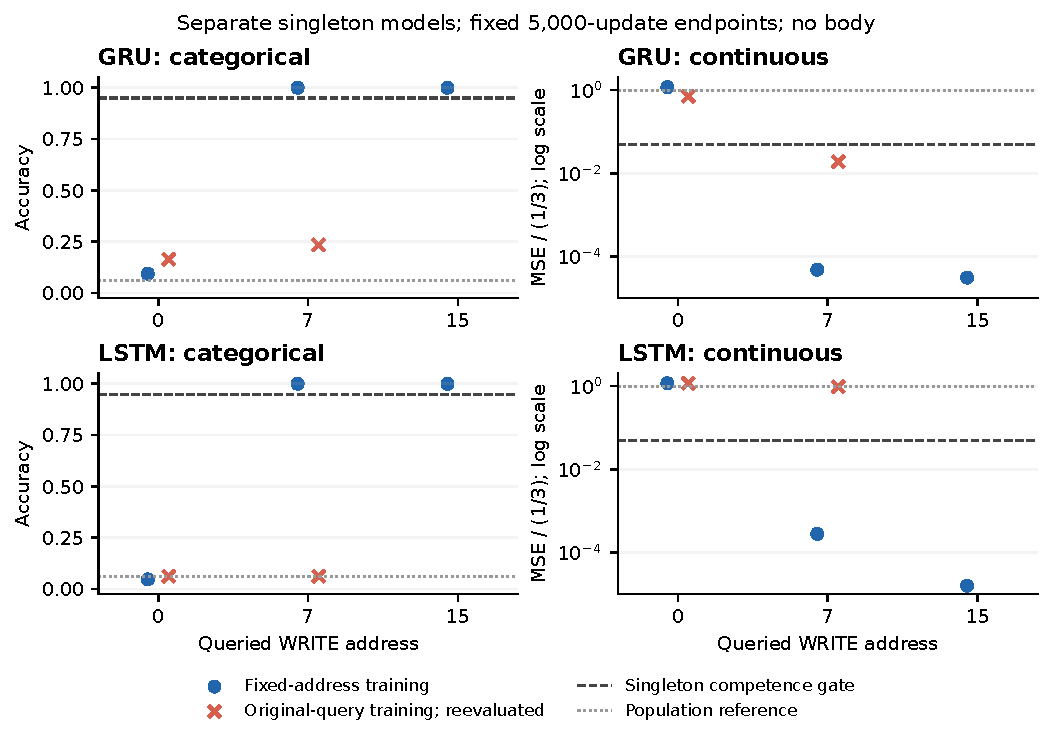
\includegraphics[width=0.92\linewidth]{../doc/auto/figures/address-acquisition-v4-endpoints.pdf}
\caption{\textbf{Singleton success does not establish joint memory competence.}
Blue points show every fixed-endpoint singleton model. All address-7 and
address-15 fits pass; all address-0 fits fail. Orange crosses reevaluate the
pinned fresh-prefix models on the same new histories at addresses 0 and 7,
without retraining. No primary baseline is supplied at address 15, outside
their original trained QUERY support. Continuous error uses a logarithmic
axis and the fixed population variance $1/3$; reference lines retain the
conventions of \cref{fig:prefix-acquisition}. Markers are offset horizontally
for visibility. There is one training seed and no trained-seed uncertainty
estimate. These are different trained weights, with no distractor body.}
\label{fig:singleton-acquisition}
\end{figure}

Categorical accuracies at addresses 0/7/15 are 0.09375/1/1 for GRU and
0.046875/1/1 for LSTM. Continuous normalized MSE is
1.171140092/0.000048020/0.000031024 for GRU and
1.169030579/0.000281015/0.000015860 for LSTM.
No address-0 scheduled checkpoint passes. The eight successful weights
cannot be combined into one model retaining all eight required items.
Address identity is confounded with 15/8/0 subsequent WRITEs, while fixed
future QUERY changes both required load and selection uncertainty.
The results therefore do not identify a pure lag, overwriting, capacity,
binding or credit-assignment effect.

This source is \hash{ab96cad9dece7d881f04065431c0d102f7665882}; the
configuration is \path{configs/experiments/address-acquisition-discovery-v4.json}.
Independent reduction reconstructs all recorded streams and 60,000 updates,
recomputes every scheduled score and supported paired error, and directly
replays a 24-checkpoint/eight-baseline subset. Complete endpoints and paired
contrasts appear in \path{doc/auto/address-acquisition-v4-results.json}.
The conditional singleton finding is accepted within this local schedule;
original eight-coordinate eligibility and periodicity harm remain unestablished.
